Our method hast to be illustrated with a simplest examples, namely three-jet production at lepton-collider $ e^+ e^- \rightarrow q + \bar{q} + g $. As in section \ref{Parton showers} shown, at first perturbative order, two Feynman diagrams contribute to the matrix element corresponding to the emission of a gluon from either the final-state quark or the anti-quark. The partonic differential cross section with respect to the quark and anti-quark momentum fractions was given by \ref{fully}:
\begin{equation}
\frac{d^2 \sigma}{dx_1 dx_2}= \hat{\sigma_0}
\frac{\alpha_s}{2\pi} C_F \frac{{x_1}^2+{x_2}^2}{(1-x_1)(1-x_2)}
\label{confi}
\end{equation}

In the parton shower approach, two contributions occur as well. For the final result, those two contributions have to be summed. 

\begin{figure}[h!]
\centering
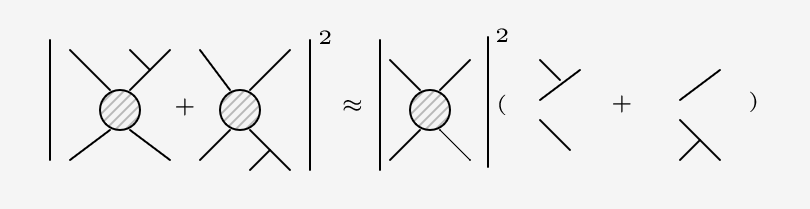
\includegraphics[width=0.85\textwidth]{images/Intro/factorization.png}
\caption{Dipole/Antenna factorisation}
\end{figure}


The dipole factorisation formula is defined by:

 \begin{equation}
 |\mathcal{M}_m+1|^2 = \displaystyle\sum\limits_{i,j} \displaystyle\sum\limits_{k\neq i,j} \mathcal{D}_{ij,k} +\displaystyle\sum\limits_{i,j} \displaystyle\sum\limits_{a} {\mathcal{D}^a}_{ij}+\displaystyle\sum\limits_{a,i} \displaystyle\sum\limits_{k\neq i} {\mathcal{D}^{ai}}_{k}+\displaystyle\sum\limits_{a,i} \displaystyle\sum\limits_{b\neq a} \mathcal{D}^{aj,b}+...
 \end{equation}
 
The calculation of the subtracted cross section involves just the evaluation of two dipole contributions from the final state emitter and final-state spectator (FF), i. e. $ D_{13,2} $ and $ D_{23,1} $. 

\begin{equation}
\begin{split}
\mathcal{D}_{13,2} (q_i,q_j,q)&= \frac{-1}{2q_i \cdot q} \:\:_2<1,\tilde{13},\tilde{2} |\frac{T_2 \cdot T_{13}}{{T_{13}}^2} V_{13,2}| 1,\tilde{13},\tilde{2} >\:_2\\
\mathcal{D}_{13,2} (q_i,q_j,q)&=\frac{1}{2p_i \cdot p_j} V_{13,2} |\mathcal{M}_{2}|^2
\end{split}
\end{equation}



\begin{equation}
\begin{split}
\mathcal{D}_{13,2} (q_i,q_j,q) &= \frac{-1}{2p_i \cdot p_j}[\frac{-(d-2)(1-z)(1-y) }{y}+\frac{(d-2)yz^2}{(1-z)(1-y)}\\
&-(\frac{-2z}{z-1}) \frac{1}{y}]|\mathcal{M}_{2}|^2
\end{split}
\end{equation}

To find the relationship between the variables, we define a total momentum $Q^{\mu} = (Q, \overrightarrow{0})$ in the Center of Mass frame.
From equation \ref{tot} can be obtained:

\begin{equation}
\begin{split}
&p_i = Q/2\:(1, \overrightarrow{0}_\bot, 1)\\
&p_i = Q/2\:(1, \overrightarrow{0}_\bot, 1)
\end{split}
\end{equation}

On the other hand, the energy fraction $ x_i $ is defined as:

\begin{equation}
\begin{split}
x_i = \frac{2 q_i \cdot Q}{Q^2}
\end{split}
\end{equation}

Therefore:
\begin{equation}
\begin{split}
x_1 = z + y(1-z)\\
x_2 = 1-y\\
x_3 = (1-z)+yz
\end{split}
\end{equation}
The addition of $x_i$ is 2 as already mentioned in section \ref{ir}.
For convenience, the shower variables are introduced expressed in terms of the $ x_i $:

\begin{equation}
\begin{split}
&\tilde{z_1}=\frac{x_1+x_2-1}{x_2}\\
&y_{13,2} =1-x_2
\end{split}
\end{equation}

For the gluon emission from the quark, after using the expressions it can be obtained \cite{Schumann:2007mg}

\begin{equation}
\frac{d^2 \sigma}{dx_1 dx_2}_{PS_q}= \hat{\sigma_0}
\frac{\alpha_s}{2\pi} C_F [\frac{1}{1-x_2} (\frac{2}{2-x_1-x_2}-(1+x_1))+\frac{1-x_1}{x_2}]
\end{equation}

For exactly the same calculating for a gluon emission of an anti-quark, it is enough to swap $ x_1 $ with $ x_2 $:

\begin{equation}
\frac{d^2 \sigma}{dx_1 dx_2}_{PS_{\bar{q}}}= \hat{\sigma_0}
\frac{\alpha_s}{2\pi} C_F [\frac{1}{1-x_1} (\frac{2}{2-x_2-x_1}-(1+x_2))+\frac{1-x_2}{x_1}]
\end{equation}

Thus, the total parton shower cross section will be:

\begin{equation}
\frac{d^2 \sigma}{dx_1 dx_2}|_{PS}=\frac{d^2 \sigma}{dx_1 dx_2}|_{PS_q}+\frac{d^2 \sigma}{dx_1 dx_2}|_{PS_{\bar{q}}}= \hat{\sigma_0}
\frac{\alpha_s}{2\pi} C_F [\frac{{x_1}^2+{x_2}^2}{(1-x_1)(1-x_2)}+\frac{1-x_1}{x_2}+\frac{1-x_2}{x_1}]
\end{equation}

Obviously, the parton shower exactly reproduces the soft and collinear singular structure of the matrix element as $ x_{1,2} \rightarrow 1 $.

Our results from the matrix of gluon radiation from an (anti)quark must actually give the same result. Unfortunately, the full calculation can not be obtained because some information from the parametrisation for the evaluation are missing, for instance $ \not{p_i} \not{m^{\mu}}_{\bot}, \not{p_j} \not{m^{\mu}}_{\bot} $. 